    \section{State-of-art}

    \pagestyle{plain}

        Nanotechnology is rapidly developing field, which is widely used in diagnostics, therapeutics and generally in biomedical research.
        Innovations in this discipline of science brings big opportunities not only for biomedicine but also for electronics, photonics, or energetics.
        There are plenty of structures, sizes, and shapes of nanoparticles (NPs) and knowledge of their sizes and shapes is crucial for their usage. \cite{35, 36, 37}

        Nano means $10^{-9}$, so the nanotechnology works with structures with size in order of nanometers. For example hydrogen atom has diameter 0.1 nm.
        If one of the dimension of the material lies between 1 to 100 nm and if it has different physical and chemical properties than bulk material.
        it is considered as nanotechnology. It stands on the border of macroworld described by classical physics and microworld described by quantum physics.
        The properties of nanomaterials can be very different than the same bulk material, it can change color, electrical conductivity, toxicity and other.
        For example solution of gold nanoparticles is red not gold. Other important parameters are that nanomaterial has far greater surface and the mass is
        so small that electromagnetic force become more important for the behavior of the particles. Anorganic nanomaterials are also able to interact
        with living systems, which has huge use in medicine. Nanomaterials can be created by two methods. The first method is called Top-down and
        starts with greater structures and ends with smaller particles. The opposite method is called Bottom-up and creates nanoparticles from single atoms.
        There are plenty of types of NPs, the most famous are carbon NPs - for example carbon nanotubes, but gold or silver NPs are also very important
        due to their properties. \cite{9, 10, 11, 12, 13, 14, 33, 34}

        Nanotechnology is quite new and developing field, first use of word 'nanotechnology' was in 1974 by N. Taniguchi. Since then nanotechnology is developing rapidly.
        But ideas, that there would be some opportunities in small world, were even earlier. In 1931 TEM (transmission electron microscopy) was created and
        in 1959 Richard Freyman, phisicist who got Nobel prize, said: 'There is plenty of room at the bottom, an invitation to enter a new field of physics.
        Nanotechnology was even used before people knew about it. For example cup from Roman empire changing color depending on angle of wiew was found.
        This was caused by nanoparticles. \cite{11, 12, 33, 34}

        Special type of NPs with huge utilization in biomedicine include surface plasmons, which are special type of electrons on the surface of NPs.
        These NPs can interact with light or generally electromagnetic radiation of wavelength much bigger than size of the NPs and localized surface
        plasmons are consequence of this radiation. This gives them outstanding optical and physical properties like strong absorption which facilitates
        using them for various optical sensors and other diagnostic methods. Localized surface plasmon resonance (LSPR) is oscillation of surface free
        electrons in spherical metal NPs and polarizing it. As a consequence induced dipole, the electron cloud is oscillating. The principle is demonstrated
        by ~\ref{fig:LSPR} Optical responses of these phenomena can be calculated from Maxwell equations. Gold NPs (AuNPs) belong to the group of plasmonic NPs
        and are used in medicine and biology due to their good chemical stability and biocompatibility. Noble metal NPs in general are also easily bioconjugated
        (conjugation with at least one biomolecule). Hence, they are a popular choice for biodetection, gene therapy for musculoskeletal regeneration,
        cancer diagnostics and therapy or Covid Antigentest. \cite{38, 39, 40, 41}

        \begin{figure}
            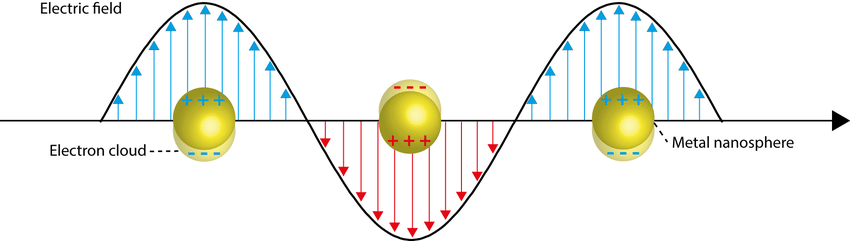
\includegraphics[width=\linewidth]{LSPR.png}
            \caption{Principle of interaction plazmon with electrical field, taken from \cite{20}}
            \label{fig:LSPR}
        \end{figure}

        This phenomena is used for plasmonic biosensors. There are two types of these biosensors, first one works on the principle of surface plasmon resonance and
        is made from thin film of noble metal. The second one uses the nanoparticles which are smaller than wavelength of light and their property of LSPR.
        Due to LSPR NPs are able to absorb and scatter light wiht high intensity. It is possible to observe it using dark-field microscopy. Thus these are highly
        applicable to biochemical sensors and cellular imaging. NPs are also useful as transducers because the scattering spectra depends on local refractive index
        and the spectra is shifted even with small changes of the refractive index. When the refractive index increases, the scaterring spectra shifts to red (bigger wavelength).
        It has also advantage in comparison with film biosensors because NPs can be used for very small volumes and gives better spatial resolution.
        The spectra of these NPs depends among other thinks on their size and shape. There are spherical NPs and nanorods which can be of various of aspect ratios (AR). \cite{1, 4, 33, 34}

        NRs are able to give two LPSRs (\ref{fig:GNR}) in comparison with spherical NPs, because the electrons can oscilate in two pathes. Oscillation of electrons inside the longer pathes
        (in longitudal dimension of the NR) is called longitudal resonance and produces light of longer wavelength, the other is called transversal resonance and
        produces light of shorter wavelength. GNR solutions can have various colors depending on their size and aspect ratio (\ref{fig:color}). \cite{4, 5, 6, 7, 8}
        For both NPs and NRs it is very important to know their sizes and shapes.
        
        \begin{figure}[h]
            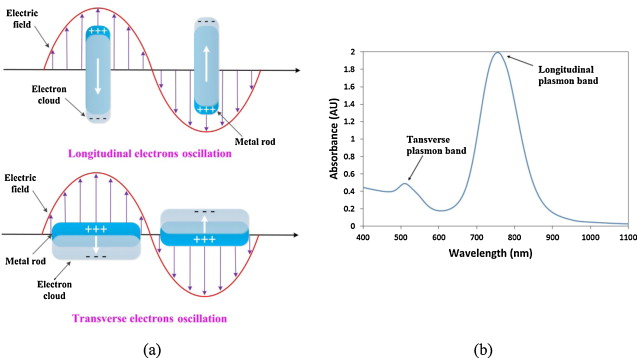
\includegraphics[width=\linewidth]{GNR.jpg}
            \caption{Principle of LPSR in GNRs, taken from \cite{19}}
            \label{fig:GNR}
        \end{figure}

        \begin{figure}[h]
            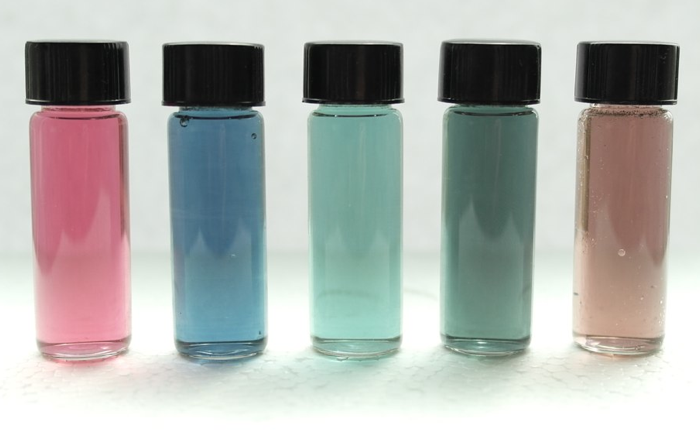
\includegraphics[width=\linewidth]{color.png}
            \caption{GNR solutions of different colors, taken from \cite{32}}
            \label{fig:color}
        \end{figure}

        One of the most common methods for determination of size and shape of AuNPs and GNRs \ref{fig:GNR_shape} is transmission electron microscopy (TEM) which is very accurate and well-known technique.
        It is just necessary to make the images of the sample and using computer count the number and size of the NPs. But there are some disadvantages. For example,
        there is the complicated and nontrivial preparation of the sample, and the measurement itself can take a long time, as well as the requirement of the actual microscope itself.
        On the other hand, it can be used for every size and shape of AuNPs and even GNRs. \cite{42}

        \begin{figure}[h]
            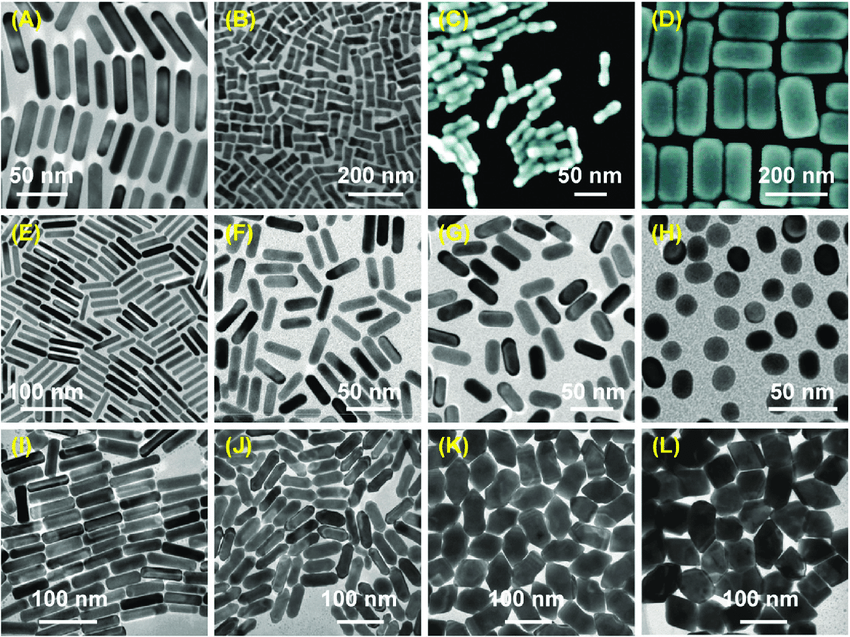
\includegraphics[width=\linewidth]{GNRs_shapes.png}
            \caption{TEM images of various shape and size GNRs, taken from \cite{20}}
            \label{fig:GNR_shape}
        \end{figure}

        The TEM microscope \ref{fig:TEM} works on the principle of electrons passing through the conductive sample and measuring the intensity of the beam that passes through.
        It consists of electron gun, system of lenses and fluorescent screen or digital detector. \cite{7}

        \begin{figure}[h]
            \centerline{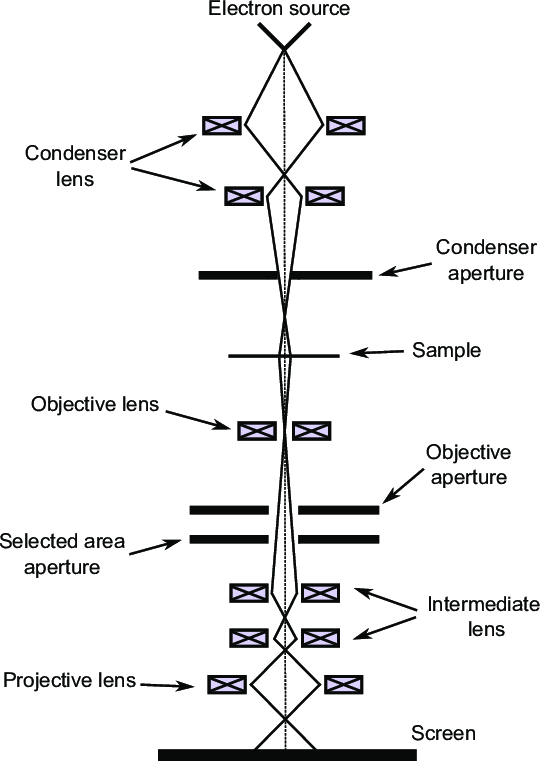
\includegraphics[width=250pt]{tem_principle.png}}
            \caption{TEM instrument schematic, taken from \cite{20}}
            \label{fig:TEM}
        \end{figure}

        The electron gun is made of cathode which is heated and has negative potential. The potential is equal to the accelerating voltage. Then the is anode with positive potential.
        The electrons come from the cathode to the anode and passes through an axial hole in the anode. Then there are condenser lenses which are used for focusing the electron beam.
        In the most cases there are two lenses. First lens reduces image and the second focuses it onto the specimen. The specimen is made by measured sample and TEM grid.
        It is situated in specimen stage which can be taken out the microscope. Then there is objective lens which produces real image and projects it onto projector lens
        which produces enlarged image. There are more than one projector lenses due to the fact that one lens can provide just magnification 5:1
        and every next lens increases the magnification range. The last step is detecting the image. There are two options. The electron beam may be absorbed on the fluorescent screen
        which produces visible light. Or it may be detected by camera and displayed on the monitor and saved as .jpg image. \cite{7}

        With TEM it is more complicated, because the result can be obtained only after image processing. It is necessary to use segmantation methods to get number, sizes and shapes of
        NPs and NRs. Segmantation is image processing technique, which transforms image into regions, each representing one object, and includes deviding objects and background.
        Image processing can be divided into three layers, segmantation belongs to low layer, then there is image analysis which belongs to middle layer and image undestanding in high layer.
        There are plenty of methods of image segmantation but it is not easy to use them. Imgage segmantation is widely used in many diagnostic systems.
        It is used for automatic evaluation and quantitative analysis of microscopic and medical images. It is crucial that the segmantation is precise, becuase if it is not,
        the algorithm will not work. Segmantation lies in finding boundaries of objects, it can be cells, anatomical structures or nanoparticles.
        But there are more steps than the segmantation, the result has to be evaluated using another algorithms. There are more types of techniques, some of them are based on
        edge detection using discontinuities in pixel values. Another techniques find similarities in regions, there are technique like region growing, clustering and thresholding.
        There are, clustering methods, connectivity-preserving techniques and region-based methods which collects regions with similar intensity, color and texture, etc. \cite{1, 2, 15, 17}

        The most basic and even fast methods are region-based methods. This group includes for example threshold segmantation and regional grown segmantation.
        First mentioned technique is very simple and fast, it just divides pixels depending on threir value. thresholding does not take in account posision of pixel,
        it works just with its intensity. There are two types of thresholds, global threshold method has same threshold value for whole image and adaptive or local
        threshold method calculates the value for each point using average region intensity. Advantige of adaptive threshold is that it accommodates to inhomogenous
        lightning of image. There are various ways how to determine threshold value. thresholding can be also divided according to how many thresholds threre are.
        Bi-level thresholding is based on one threshold and divides pixels into two groups and multilevel thresholding selects multiple thresholds, thus there are several groups of pixels.
        One of the most used methods is called Otsu threshold \ref{fig:otsu} and consist in finding value, where weighted within class variance is minimal. This method expects that histogram of image
        is bimodal, it means there is sufficient difference between background and region of interest intensity. \cite{15, 16, 17, 18}
        
        \begin{figure}[h]
            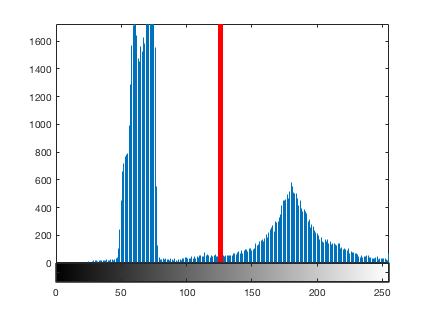
\includegraphics[width=\linewidth]{otsu_method.png}
            \caption{otsu threshold in bimodal histogram, taken from \cite{20}}
            \label{fig:otsu}
        \end{figure}

        There are also entropy-based techniques. Entropy is originally
        used in thermodynamics and it describes level of disorder of physical system. Shannon described entropy in informatics as unit for measuring efficiency of information in system.
        Entropic thresholding works on principle of finding threshold where sum of entropy of background and entropy of ROI is maximal. Another method is called minimum error thresholding
        and it considers histogram as probability density function which includes combination two populations, intensity of ROI pixels and of background pixels and
        it determines threshold as value, where overlap of these two population is minimal. It uses estimation of parameters of mean value, standard deviation and probability.
        This algorithm works with 2-D histogram, which can show relatiionship between two variables. There is also 2-D minimum error method which takes in account also position of pixel.
        multilevel thresholding determines more that one threshold and divides image into more levels depending on intensity and color (in RGB images). It is ideal for images with color
        inhomogenous background. Thus it is possible for example to assign both dark and bright pixels to zero and middle gray pixels to one. disadvantage of these algorithms is
        it is often not possible to detect number of thresholds automatically. There are methods which can determine it using several times lowpass or highpass filters in image histogram
        to decrease or incease number of local maxina and minima.
        Another region-based type of image segmantation algorithms is called regional growth segmantation. It assumes that pixels of one region have similar values. Algorithm first selects
        seed pixel and then join similar pixels in neiborhood connected with this pixel into the region. It requires threshold value which is used as maximum difference between seed pixel
        and pixels assigned to the region. Disadvantage of these method is that it is slow and susceptible to noise. \cite{15, 16, 17, 18}

        Another segmantation algorithm is called watershed segmantation algorithm (\ref{fig:watershed}) and is also region-based method. The name and even principle comes from nature and it is applied
        to grayscale or binary images. The goal of this algorithm is to find all connections in the image. connected pixels mean pixels that create one object (for example nanoparticle).
        First step of binary image works on principle of distance from nonzero pixel which creates distance map. Objects have to be of value zero and background of zero one,
        if it is reverse, image has to be negated first. In case of grayscale images the distance is calculated from local minima. So objects have to be of lower value than background.
        When distance map is calculated, watershed transform can be applied, it starts filling pixels from the highest value of distance and stops before two connected object join into one.
        It is called decomposition into catchment basins. Basins represente individual objects or regions. Every pixel of image is classified into one of the region or to background,
        so noise can be problem, because it creates large number of small regions. It is called over-segmantation. Thus image has to be filtered before applying watershed transform.
        \cite{2, 3}
        
        \begin{figure}[h]
            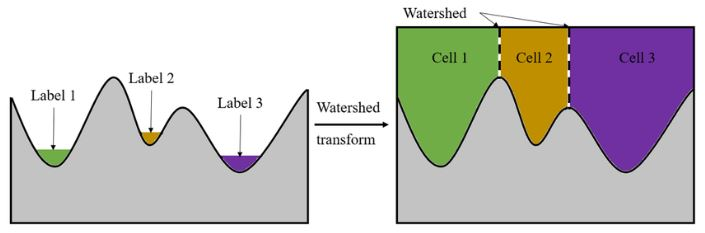
\includegraphics[width=\linewidth]{watershed.jpg}
            \caption{Watershed principle, taken from \cite{20}}
            \label{fig:watershed}
        \end{figure}

        Edge detection technique works on principle of finding local changes and discontinuities in the image \cite{22}. It works with spatial domain instead of histogram in contrast with thresholding.
        Edge detection means detecting high frequencies in image, so it works like high-pass filter. Spatial frequency is generally number of cycles per distance, it has two components,
        frequency in x axis and y axis. In images it has units pairs of lines per milimeter, it means how quickly low value pixels shifts changes with high value pixels.
        This spectra can be obtained using discrete 2D Fourier transform, which is function of x and y. Thus high-pass filter extracts high frequencies and low-pass filter low frequencies \cite{23}.
        There are four types of edges, step edge where the value changes from one pixel to another, ramp edge, where the change is more gradual. Line edge have steep change
        but then returns to original value. Roof edge is made of slow change and in the peak value it also slowly returns back to original value.
        There are more steps in edge detection algorithm, filtering is used for removing noise. For example salt and pepper noise
        which means random white and black pixels in the image. It has to be very well balanced because filtering also reduces edge strange.
        Then there is enhancement phase which points up pixels with greater change of value. This step uses calculating gradient. Last step is called detection
        and it removes pixels with nonzero gradients which are nor edges. \cite{3} Greater changes of value can be detected using differential operators which can calculate derivatives.
        There are several types of these descrete operators, Sobel and Laplacian operators are of the most used. Sobel operator calculates first derivative in each pixel.
        Tha algorithm uses two 3x3 matrices, transverse matrix which founds gradients in horizontal direction and longitudal matrix which founds gradients in vertical direction \cite{17, 22}.
        Then size of gradient is calculated using equation:

        \begin{equation}
            G = \sqrt{G_x^2 + G_y^2}
        \end{equation}
        \cite{22}
        
        And vector of gradient can be calculated using equation:

        \begin{equation}
            \Theta = \arctan{\frac{G_x}{G_y}}
        \end{equation}
        \cite{22}

        Zero angle corresponds with longitudinal edge, where pixels in left have lower value than ones in right.

        \begin{figure}[h]
            \centering
            \begin{bmatrix}
                -1 & 0 & 1\\
                -2 & 0 & 2\\
                -1 & 0 & 1
            \end{bmatrix}\hlinefill
            \begin{bmatrix}
                1 & 2 & 1\\
                0 & 0 & 0\\
                -1 & -2 & -1
            \end{bmatrix}
            \caption{Sobel operators, horizontal and vertical \cite{22}}
        \end{figure}

        Another type of differential operator is called Laplacian operator and it is operator of second derivative and it detects zero-crossing of image intensity. It is more accurate
        than Sobel operator, but it detects isolated pixels better than edges, so it is not possible to use it to images with noise \cite{22}. Thus before using Laplacian operator it is
        necessary to perform low-pass filter, which reduces noise. For example median filter can be used, because it reduces noise while keep sharp edges.
        It is also possible to combine it with edge-matching filter, which has minimal response to isolated pixels and good response to merged edges \cite{21}. Due to this disadvantage,
        Laplacian operator is not frequently used. It consist from only one symetric matrix thus it is used for both directions. It can be also calculated using equation:

        \begin{equation}
            \nabla^2f = \frac{\partial^2f}{\partial x^2} + \frac{\partial^2f}{\partial y^2}
        \end{equation}
        \cite{22}

        \begin{figure}[h]
            \centering
            \begin{bmatrix}
                0 & 1 & 0\\
                1 & -4 & 1\\
                0 & 1 & 0
            \end{bmatrix}
            \caption{Laplacian operator \cite{22}}
        \end{figure}

        Clustering techniques work on principle of deviding pixels into various groups (clusters) depending on their characteristics. Cluster can be defined as group of pixels
        with similar properties with each other in same cluster and diverse with each other clusters \cite{26}. There are two types of clustering algorithms, hierarchical clustering
        is based on merging pixels with similar characteristics or spliting pixels with opposite characteristics and finds all possible combinations. Partitional clustering
        is iteration method with successive optimalization. hierarchical clustering can be divided into two groups, first is called agglomerative or bottom-up method and
        works on principle of merging data based on their similarities, first it defines every pixel as one cluster and then in every iteration merges similar clusters into one, until
        it reaches given number of clusters. Divisive or top-down method takes all pixels into one cluster and then in every cycle divides the most diverse pixels and from each clusters
        creates two \cite{25, 26} One of the most used clustering method is called k-means \ref{fig:k-means} and comes under partitional methods. Advantige of this method is that it is easy, fast and results are
        of high quality. Algorithm first randomly selects defined number (k) of cluster centers and assigns each pixel to the nearist cluster. In every iteration algorithm
        calculates for every cluster new center using mean value of all pixels in this cluster and then reallocates pixels depending on new distances from centers.
        Algorithm finishes when there is no significant change in centers \cite{26}. disadvantage of this method is that it is difficult to estimate k parameter.

        \begin{figure}[h]
            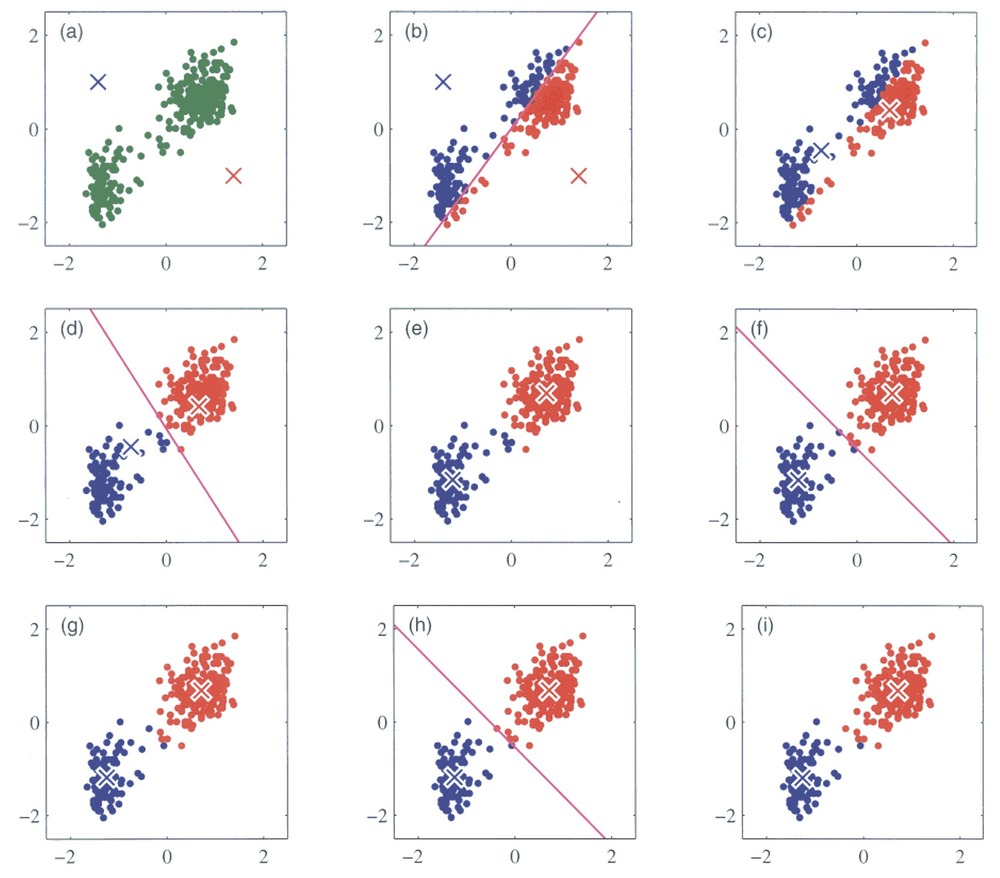
\includegraphics[width=\linewidth]{k-means.jpg}
            \caption{K-means principle, taken from \cite{24}}
            \label{fig:k-means}
        \end{figure}

        Another iterative algorithm is called fuzzy C-means clustering. It is based on fuzzy sets which does not assign each point just into one cluster, but instead of this,
        it calculates vector of memberships for each pixel, it means how strongly it belongs to each cluster. It has to be numbers between 0 and 1, sum of all memberships of one pixel must be 1.
        It is advantige in compare with k-means, because it allows overlapping of clusters. There si also defined number of clusters (c). Steps of C-means is similar as k-means,
        algorithm first randomly selects c centers, then calculates membership and updates cluster centers. Disadvantage is the same as in k-means,
        it is necessary to specify C parameter \cite{26, 27, 28}. There are more clustering algorithms, for example Gaussian clustering, but it has disadvantage, that is very complex.
        It is also iterative method and works on principle of calculating probability \cite{27}.

        There are also image segmantation techniques which use deep learning, wchich is subset of machine learning using neural network architecture with many layers.
        These systems requires large number of sample images and very good computating power. In biomedicine it is udes for example for automatic detectiion of cancer cells.
        Each neural network is composed from input layer, some amount of hidden layers and output layer. Deep learning neural networks may contain about 150 hidden layers
        in compared with traditional neural networks, wchich have 2-3. It can also learn automatically just from large datasets (2). Neural networks are formed from
        nodes which are connected with other nodes, these nodes are called neurons \ref{fig:neural_networks}. Each connection has weight, thus some of them are more important than others \cite{29}.
        Output of neuron can be calculated using equation:

        \begin{equation}
            y = f(\sum_{i=0}^{p} w_i x_i - \Theta)
        \end{equation}

        where \(y\) is output, \(x_i\) is i-th input, \(w_i\) is weigth of i-th input, \(f\) is activation function and \(\Theta\) is threshold of neuron \cite{29}.

        There are two types of operations, output of neuron can be linear function of weighted sum of inputs which in each connection multiplied by weight, the bigger is input,
        the bigger is output. Or there can be threshold and if weighted sum of inputs reaches this value, neuron becomes active and there is signal, which is multiplied in each
        connection with weight, otherway there is no signal. \cite{29}.

        \begin{figure}[h]
            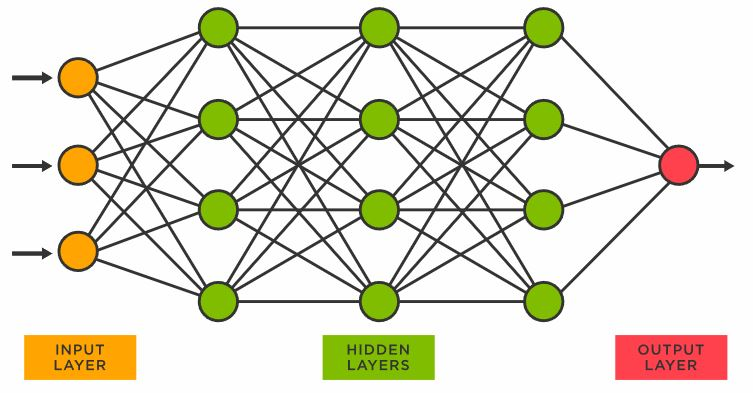
\includegraphics[width=\linewidth]{neural_network.jpg}
            \caption{Neural networks layers, taken from \cite{20}}
            \label{fig:neural_networks}
        \end{figure}

        Artificial neural network (ANN) is basic model of deep neural networks. It is composed of perceptrons, which means that signal moves just forward and output is connected to output.
        it uses back-propagation (feedback) to reduce errors while learning, during this it updates weights of connections. it is called adviser learning. \cite{30}
        Convolutional neural networks (CNN) are types of deep neural networks wchich are used for images, because it contains 2D layers. Ii learns directly from sample images \cite{2}.
        In CNN signal moves just forward thru all the hidden layers and output is connected with input thru these layers.
        CNN have three types of hidden layers, convolutional layer, which contains convolution of kernel matrix, which includes learned parameters, ant the image, it creates new matrix
        called activation map. This operation is applied by each layer in this group. pooling layer which merges each region into one value, there are more methods of this pooling function,
        it can be mean value, weighted value depending on distance from center pixel of region or max value of region, it reduces size of output thus computational complexity is decreased.
        Then there is fully connected layer, which connects all neurons from previous with each neuron from following layer. Then there usually are also nonlinear layers placed
        after convolutional layer,this layer uses non-linear operators to activation map. Prerequisite for this method is large number of relevant sample labeled images for training. \cite{30, 31}
        Recurrent neural network (RNN) are not feed-forward neural network, it means signal does not move just forward like in ANN and CNN. There is recurrent path which is able to affect input.
        it is connected with feedback, which figures like memory which connects sequence of data. RNN works previous data, so it can take it in account and output depends on it.
        These sequences of data represent in image processing spatial domain. \cite{30}

    \clearpage	
    \renewcommand{\refname}{Reference} 	% Přejmenování Reference
    (Nepodařilo se mi najít bibTex citace pro jiné zdroje než články, zatím jsem vložila jen ISBN pro knihy
    a odkazy pro webové stránky, do finální verze projektu to doplním.)
    \printbibliography
    \clearpage

\end{document}